\chapter{Aproximação de Problemas de Valores Iniciais (PVI's): Implementação e Exemplos}

    \label{cap:aproxPVI}

    As equações diferenciais ordinárias podem ser solucionadas 
    analiticamente usando-se ou a integração ou o método dos fatores integrantes ou séries de potências ou a transformada de Laplace, 
    dependendo de sua forma. Esses métodos de resolução de EDO's não serão apresentados aqui, por fugirem 
    ao escopo desse trabalho, mas o leitor pode se inteirar sobre eles, podendo encontrar 
    informações bem fundamentadas e diversos exercícios em \cite{boyce9, regiIntro}.
    
    Esse trabalho visa o uso de métodos numéricos para a aproximação de PVI's (e também, rapidamente, PVC's). 
    Dentre os métodos para resolução de PVI's, destacam-se o método de Euler e os métodos de Runge-Kutta 
    (no caso desse trabalho, o de 4ª ordem). Para a resolução de PVC's pode-se usar o método de Diferenças
    Finitas, por exemplo, a ser visto mais a frente.
    
    \section{O Método de Euler}
    
        Esse é um método pouco usado na prática para a aproximação de PVI's \cite{burden} devido a sua alta divergência 
        do resultado real após algumas iterações. Entretanto, por poder ser facilmente explicado e por suas variações 
        serem utilizadas para a finalidade deste trabalho, será definido aqui esse método.
        
        Seja um PVI como o da Seção \ref{PVIsec} e seja $y(t)$ a solução desse PVI. Podemos
        representar qualquer função por uma série de Taylor como
		\begin{equation}
		    \label{TayPol}
			T_{n}(x) = \sum_{j=0}^{n} \frac{f^{(j)}(c)}{j!}(x - c)^{j}
		\end{equation}
        Seja então
        \begin{equation}
            \label{TayExpYt}
            y(t) = y(t_0) + hy'(t_0) + \dfrac{h^2}{2}y''(t_0) + \dfrac{h^3}{6}y'''(t_0) + \cdots
        \end{equation}
        a expansão da solução $y(t)$ em série de Taylor em torno do valor inicial $t_0$ e sendo $h$ o passo usado para a geração dos 
        valores de $t$.
        
        Se truncarmos (\ref{TayExpYt}) logo depois do termo da primeira derivada, tendo $t_1 = t_0 + h$ e $y_1$ como a aproximação
        de $y(t_1)$, além de se saber que $y' = f(t, y)$, temos que
        \begin{equation*}
            y_1 = y_0 + f(t_0, y_0)
        \end{equation*}
        Logo, as aproximações $y_i$ de $y(t_i)$ podem ser obtidas semelhantemente à forma da equação anterior \cite{fred}
        \begin{equation}
            y_{i+1} = y_i + hf(t_i, y_i) 
        \end{equation}
        
        Um código em Python para o método de Euler, baseado no algoritmo de Frederico \cite{fred}, seria
        \lstinputlisting[caption=Método de Euler]{Codigos/euler.py}
    
    \section{O Método de Runge-Kutta}
    
        Segundo Burden \cite{burden}, os métodos de Runge-Kutta apresentam a vantagem, em relação aos Taylor, de não necessitarem do cálculo das derivadas de
        uma função $f(x, y)$, além de terem o erro de truncamento local de alta ordem .

        O método de Runge-Kutta de quarta ordem (RK4) consiste em um sistema não-linear com 11 equações e 13 incógnitas. Essas equações podem ser obtidas de forma semelhante a obtenção do método de Euler, através da expansão e truncamento de um polinômio de Taylor para uma função $f(x, y)$ \cite{fred}. O método é definido por
        \begin{align}
            y' &= f(y(t), t) \\%\text{, com y(t_0) = y_0} \\
            K_1 &= f(y^*(t_0), t_0) \\
            K_2 &= f(y^*(t_0) + \dfrac{h}{2}K_1, t_0 + \dfrac{h}{2}) \\
            K_3 &= f(y^*(t_0) + \dfrac{h}{2}K_2, t_0 + \dfrac{h}{2}) \\
            K_4 &= f(y^*(t_0) + hK_3, t_0 + h) \\
            y^*(t_0 + h) &= y^*(t_0) + \dfrac{h}{6}(K_1 + 2K_2 + 2K_3 + K_4)
        \end{align}
        com $y(t_0) = y_0$.
        
        Um código em Python para esse método pode ser visto abaixo:
        \lstinputlisting[caption=Método de Runge-Kutta de quarta ordem (RK4), firstline=5, label=RK4]{Codigos/RK4.py}
        
        O código acima é utilizado nesse trabalho como uma ferramenta para a resolução de EDO's que serão apresentadas no Capítulo \ref{cap:RT}, além é claro, de usá-lo na demonstração de exemplos da resolução numérica de EDO's pelo mesmo. 
        
        Basta importá-lo no código em que se deseja usá-lo e realizar a chamada da função \textit{rungeKutta4Ordem}, passando-se os devidos parâmetros a ele. Dentre esses parâmetros, se encontra um por nome \textit{EDO}, que é um objeto da classe \textit{EqDiferencialOrdinaria} (cuja definição é apresentada na próxima seção), que representa a EDO a ser resolvida pelo método.
        
    \section{Exemplos de Resoluções de PVI's Usando o RK4}
        O código a seguir abstrai uma ou mais EDO('s) computacionalmente. Assim como o código apresentado para o método de Runge-Kutta de 4ª ordem, apresentado na seção anterior, esse código pode ser chamado por um programa.
        
        \lstinputlisting[caption=Classe abstrata que define uma equação diferencial ordinária de forma básica]{Codigos/eqDiferencialOrdinaria.py}
        
        A função abstrata (que tem apenas a sua assinatura definida, não sendo implementada em primeiro momento) \textit{evaluate} tem seu código escrito pelo programa que a chama, visto que cada EDO apresenta um comportamento próprio.
        
        \subsection{Modelo de Crescimento Populacional de Malthus}
        
            Usado na área da ecologia e nos estudos sobre dinâmica populacional, o modelo descrito por Malthus
            \begin{equation}
                \begin{cases}
                    \dfrac{dy}{dt} = ky\\
                    y(t_0) = y_0
                \end{cases}
            \end{equation}
            no qual $k$ representa a taxa de crescimento populacional e $y_0$ é a população existente no tempo $t_0$, diz que a taxa de crescimento populacional $y'(\dfrac{dy}{dt})$ é proporcional à população existente $y$ naquele instante $t$. Sua solução analítica é $y(t) = y_0e^{kt}$ \cite{regiIntro, Malthus}.
    
            Como exemplo de resolução numérica, por meio do método de Runge-Kutta, para esse modelo apresentamos o seguinte código. Seja a equação diferencial
            \begin{equation}
                \label{eq:exMalthus}
                \dfrac{dy}{dt} = e^t
            \end{equation}
            (cuja solução analítica é $y(t) = e^t$). 
            
            O código a seguir realiza um resolução numérica para esse problema de Malthus utilizando o método de Runge-Kutta de 4ª ordem. A classe \textit{EqMaltus} extende a classe \textit{EqDiferencialOrdinaria}, definindo a função \textit{evaluate} para retornar $e^t$. São pedidos 50 passos e parte-se do instante $t = 0,0$.
            \lstinputlisting[caption=Resolução por RK4 da equação \ref{eq:exMalthus}, firstline=36]{Codigos/testeMaltus.py}
            
            O gráfico gerado com o auxílio desse código é
            \begin{figure}[H]
                \centering 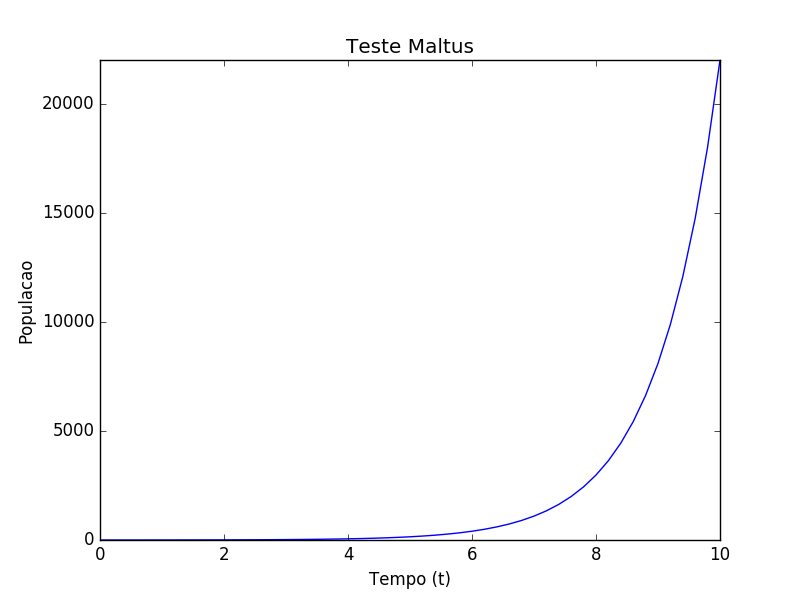
\includegraphics[width=10cm,height=6cm]{resultsCodigos/testeMaltus.png}
                \caption{Resolução numérica do problema \ref{eq:exMalthus}}
                \label{fig:Malthus}
            \end{figure}
            Como podemos ver, a resolução numérica condiz com a solução analítica exponencial.
    
        \subsection{Equações de Lotka-Volterra}
        
            \subsubsection{Definição}
            
        		As equações de Lotka-Volterra foram propostas pelo matemático Vito Volterra e pelo biofísico Alfred J. Lotka no ano de 1925. Elas são um par de equações diferenciais não-lineares e de primeira ordem.
        		 
        		As equações de Lotka-Volterra são mais utilizadas em quadros biológicos envolvendo presas e predadores (como lobos e ovelhas ou golfinhos e peixes), sendo a população das presas considerada a única fonte de alimento para a população de predadores e que não há competição entre os predadores. 
        		
        		Como descrevem um quadro simples, essas equações, em sua definição, não proporcionam uma análise muito próxima da realidade, mas o entendimento sobre elas possibilita o entendimento de situações mais complexas.
		
	        \subsubsection{Principais Situações Descritas pelas Equações}
        		
        		Por suas relações diretas com o contexto de presa-predador, as equações de Lotka-Volterra podem descrever as seguintes situações
		
        		\begin{itemize}
        			\item Extinção de predadores;
        			\item Extinção de presas;
        			\item Existência de predadores e presas ao mesmo tempo;
        			\item Geral.
        		\end{itemize} 
	
        		Cada uma dessas situações para as equações será demonstrada a seguir, considerando $x$ como o número de indivíduos para a população de presas, $y$ para o número de indivíduos da população de predadores e $t$ para o tempo.
		
		    \subsubsection{Caso 01: Extinção de Predadores}
    			
    			Caso $y = 0$ (população de predadores extinta), a população de presas cresce proporcionalmente à população atual, o que é representado por $k$
    			
    				\[y = 0\]
    				
    				\[\frac{dx}{dt} = kx\ \text{, }\qquad k > 0\]
				
		    \subsubsection{Caso 02: Extinção de Presas}
			
    			Caso $x = 0$, ou seja, a população de presas seja extinta, a população de predadores deve se extinguir também, visto que as presas citadas no problema são sua única fonte de alimento. Esse decrescimento na população de predadores se dá proporcionalmente à população atual, sendo tal proporção representada por $r$
    			
    				\[x = 0\]
    				
    				\[\frac{dx}{dt} = - ry \text{, }\qquad r > 0\]
				
		    \subsubsection{Caso 03: Existência de Predadores e Presas ao Mesmo Tempo}
		    
    			Diz-se que as situações em que presa e predador se encontram levam à morte de uma presa e as ocorrências de tais situações são proporcionais ao produtos das populações de presas e predadores. Essa situação é modelada utilizando-se duas constantes de proporcionalidade: $a$ para a taxa de predação e $b$ para a conversão de presa para predador. Logo:
    			
    			\begin{itemize}
    				\item População de presas sofre queda: $-axy$
    				\item População de predadores aumenta: $bxy$
    			\end{itemize}
		
		    \subsubsection{Caso geral}
		    
    			Considerando todos os três casos acima em conjunto, tem-se:
    			
    				\[\frac{dx}{dt} = x (k - a y)\]
    				
    				\[\frac{dy}{dt} = y (r x - b)\]
    			onde $k, a, b \text{ e }r$ relacionam as duas populações.
			
        	\subsubsection{A Relação Entre as Equações de Caso Geral e sua Solução Geral}
	
        		Relacionando ambas as equações de caso geral, encontra-se
        		
        			\[\frac{dy}{dx} = \frac{y (r x - b)}{x (k - a y)}\]
        		cuja solução geral, a partir de integração, é
        		
        			\[k ln(y) - a(y) + C = -b ln(x) + b(x) + D\]
        		sendo C e D constantes de integração \cite{wiki:eqLotkaVolterra}.
        		
        	\subsubsection{Implementação}
        	
        	    O código a seguir propõe uma resolução para um problema de equações de Lotka-Volterra do livro Cálculo, vol. 2, de James Stewart \cite{stewart}. Nesse exemplo, temos que as equações regem as populações de presas e predadores tendo-se
        	    \begin{align*}
        	        k &= 2,0\\
        	        a &= 0,01\\
        	        r &= 0,5\\
        	        b &= 0,0001
        	    \end{align*}
        	    sendo sua condição inicial $t = 0,0$ com 2000 presas e 35 predadores.
        	    
        	    Espera-se que os resultados exibam oscilações entre as populações de presas e predadores. A medida que a população predatória cresce, a de presas deve cair, levando também a predatória a queda, o que fará a de presas subir. Isso deve se dar em ciclos.
        	    
        	    \lstinputlisting[caption=Problema envolvendo as equações de Lotka-Volterra \cite{stewart}, label=LK,firstline=45]{Codigos/testePresaPredador.py}
        	    
        	    \begin{figure}[H]
        	        \centering 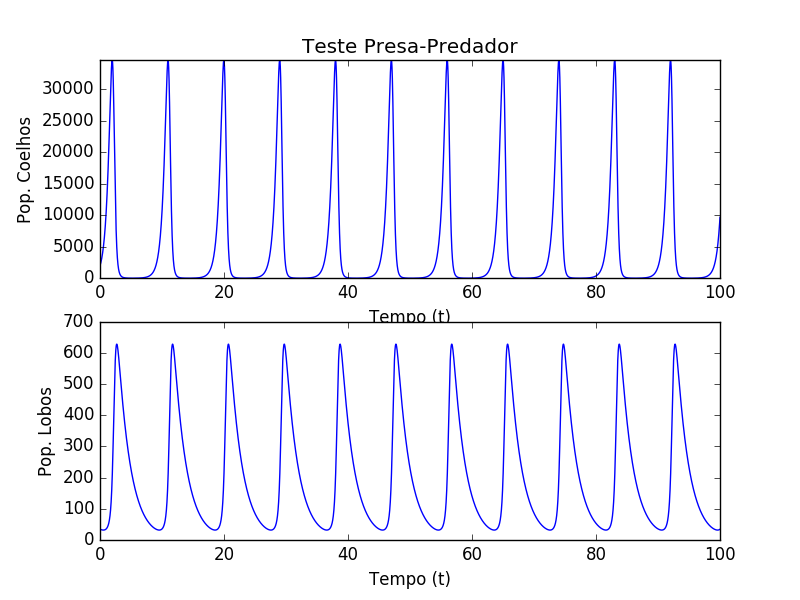
\includegraphics[scale=.8]{resultsCodigos/testePresaPredador.png}
        	        \caption{Resultado do código \ref{LK}}
        	        \label{fig:testPresaPredador}
        	    \end{figure}
        	    
        	    A Figura \ref{fig:testPresaPredador} ilustra, quantitativamente, as populações de joaninhas (predadores) e pulgões (presas) ao longo do tempo $t$. Podemos perceber que logo após a população de presas atingir seus picos, a população de predadores cresce e aplaca as presas, cuja população quase se anula. Com essa rápida queda, a população de predadores tende a decrescer também. Esse processo se repete ao longo do tempo.
        	    
        	    Nesse tipo de problema, as populações de presas e predadores podem sofrer influência de fatores externos também, como o clima. Sendo $\omega$ a frequência da interferência do clima sobre a população de presas, $\alpha$ a amplitude dessa interferência e $\beta$ a média dessa população ao longo do tempo, podemos modelar a influência $K$ do clima sobre a população de presas ao longo do tempo pela equação
        	    \begin{equation}
        	        K(t) = k(1 + \alpha\sin{\omega t} + \beta)
        	    \end{equation}
        	    cujo código em Python se dá por 
        	    
        	    \lstinputlisting[caption=Definição da influência do clima sobre a população de presas ao longo do tempo]{Codigos/influenciaClima.py}
        	    
        	    dentro do método \textit{evaluate} do Código \ref{LK}
        	    
        	    Para esse caso de influência pelo clima obtemos um resultado como da Figura \ref{fig:LCK}. Nele, percebemos que as altas da população de presas se dão próximas à média da variação climática. Crescendo a população de presas, começa a crescer a população predatória, que causa um decrescimento drástico na primeira. Isso leva a população de predadores a decrescer também.
        	    
        	    \begin{figure}[H]
        	        \centering
        	        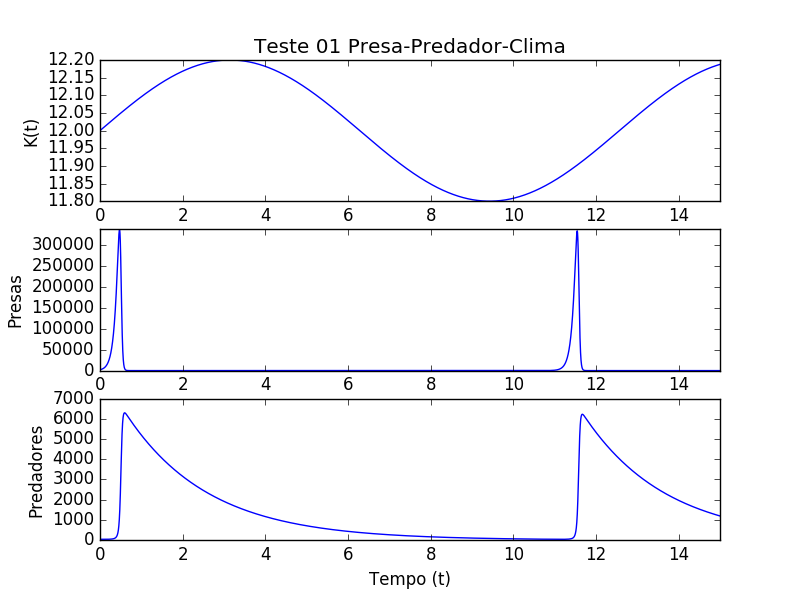
\includegraphics[scale=.6]{resultsCodigos/testePresaPredadorClima01ParaTmax100.png}
        	        \caption{Relação de presas e predatores agora influenciada pelo clima}
        	        \label{fig:LCK}
        	    \end{figure}
    
        \subsection{Sistema Massa-Mola}
        
            Seja um corpo de massa $m$ conectado a uma mola de constante elástica $k$ como na Figura \ref{fig:massaMola}. Esse conjunto é nomeado \textbf{Sistema Massa-Mola}.  
            Os experimentos envolvendo este sistema, em geral, consistem em tirar o conjunto de seu repouso e iniciar sua oscilação, medindo-se então as posições e velocidades do corpo durante as oscilações.
            \begin{figure}[H]
                \centering
                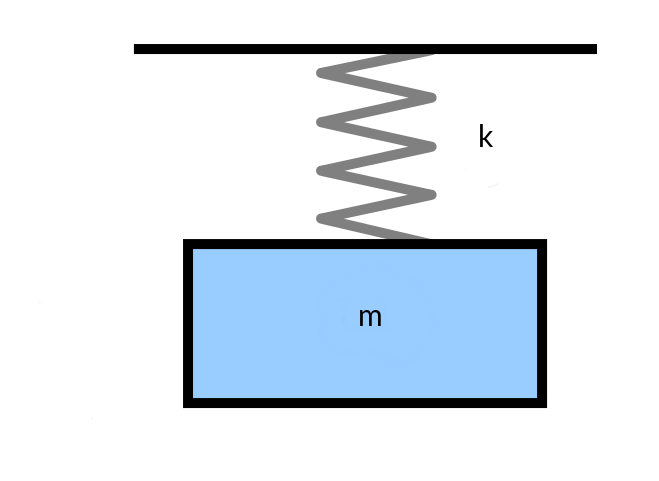
\includegraphics[scale=.25]{imagens/Mass_spring.png}
                \caption{Sistema massa-mola}
                \label{fig:massaMola}
            \end{figure}
            
            O sistema vertical possui três forças agindo sobre ele: a força peso, que podemos nomear por $P$, apontando para baixo, a força elástica da mola, que podemos nomear por $F_e$ e a força de resistência, que nomeamos por $F_r$. $F_e$ última aponta para a direção contrária ao movimento da massa. Essas forças podem ser descritas pelas seguintes equações
            \begin{align}
                P &= mg\\
                F_e &= -ky(t)\\
                F_r &= \gamma y'(t)
            \end{align}
            sendo $g$ a aceleração da gravidade, $y(t)$ o deslocamento feito na mola, $\gamma$ a constante de amortecimento (resistência do ar) e $y'(t)$ a velocidade das oscilações na mola.
            
            Pode haver ainda uma quarta força atuando sobre o sistema: a força externa representada por $F_{ext}$. Essa pode representar, por exemplo, um pistão conectado à mola, que fica gerando outras oscilações no sistema (como veremos na próxima subsubseção) ou, simplesmente, a força gravitacional, como escolhemos para este caso.
            
            Se adotarmos o sistema cartesiano como referencial (termos positivos apontam para cima ou direita, termos negativos apontam para baixo ou esquerda) temos que, pela segunda Lei de Newton
            \begin{align}
                \label{Newton2}
                F &= ma\\
                \intertext{escrevemos a aceleração na forma de derivada}
                F &= my''(t)\\
                \intertext{definimos a força resultante ($F = my''(t)$) como o somatório das forças atuantes sobre o sistema, considerando o sentido das mesmas}
                my''(t) &= F_e + F_r - P\\
                \intertext{substituímos cada força atuante por suas fórmulas}
                \label{eqDifOsc}
                my''(t) &= -ky(t) + \gamma y'(t) - mg\\
                \intertext{isolamos a força externa no lado direito da equação}
                my''(t) - \gamma y'(t) + ky(t) &= -mg
            \end{align}
            essa última equação, satisfeita por $y(t)$ descreve o movimento da massa durante as oscilações do sistema. Nesse tipo de equação, que descreve um comportamento oscilatório, o termo direito representa a força externa $F_{ext}$ que age sobre o sistema. Nesse caso, podemos perceber que $F_{ext}$ é a força gravitacional e que seu sinal negativo indica que ela está apontando para baixo.
            
            O coeficiente $\gamma$ que multiplica $y'(t)$ representa o amortecimento do sistema massa-mola. Empiricamente, o amortecimento pode se dar por um líquido colocado abaixo da massa ou pelo atrito da massa com o ar, por exemplo. O sistema também pode ser considerado sem amortecimento ($\gamma = 0$), o que significa que ele oscilará permanentemente. Mais detalhes sobre o amortecimento desses sistemas podem ser encontrados em \cite{boyce9, regiIntro}.
            
            A solução analítica geral desse sistema é 
            \begin{equation}
                u(t) = c_1\cos{\omega t} + c_2\sin{\omega t}
            \end{equation}
            na qual, $c_1$ e $c_2$ são constantes e $\omega_0$ é a frequência natural dada por $\sqrt{\dfrac{k}{m}}$ do sistema \cite{regiIntro}.
            
            O exemplo a seguir resolve um sistema massa-mola amortecido descrito por 
            \begin{equation*}
                s'' + 0,125s' + s = 0
            \end{equation*}
            com condições iniciais $t = 0.0$, $V_0 = 0.0$ e $P_0 = 2.0$, sendo que $V_0$ e $P_0$ representam, respectivamente, a velocidade e a posição inicial da massa no sistema.
            \lstinputlisting[firstline=45,caption=Código da resolução numérica de um problema envolvendo um sistema massa-mola amortecido]{Codigos/testeMassaMola.py}
            cujo resultado é exibido na figura \ref{fig:MMamortecido}
            \begin{figure}[H]
                \centering
                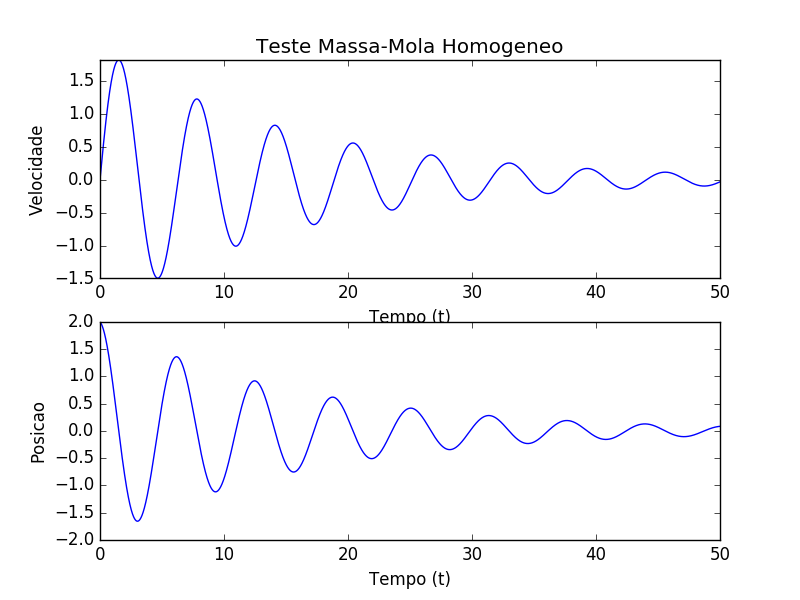
\includegraphics[scale=.54]{imagens/testeMassaMola.png}
                \caption{Gráficos da posição e da velocidade da massa do sistema ao longo do tempo}
                \label{fig:MMamortecido}
            \end{figure}
            
            No primeiro gráfico da Figura \ref{fig:MMamortecido} vemos o gráfico da velocidade da massa em cada instante de tempo.
            Podemos perceber o efeito do amortecimento sobre o sistema pela diminuição da amplitude do movimento e da velocidade dele ao longo do tempo.
            
            \subsubsection{Sistema Massa-Mola Forçado}
    
                Suponha que a força externa $F_{ext}$, que em (\ref{eqDifOsc}) era $-mg$ dependesse do tempo $t$ e fosse periódica, como um pistão que forçasse a mola de um lado para o outro. Teríamos então um \textbf{Sistema Massa-Mola Forçado}, como na Figura \ref{fig:forcedMMS}, no qual $F_{ext} = F_0\cos{\omega t}$, sendo $F_0$ é amplitude da força periódica e $\omega$ é a frequência dela. Nesse sistema ocorre um movimento chamado \textbf{batimento}, que é uma oscilação com uma frequência cuja amplitude também oscila \cite{regiIntro}.
                
                \begin{figure}[H]
                    \centering
                    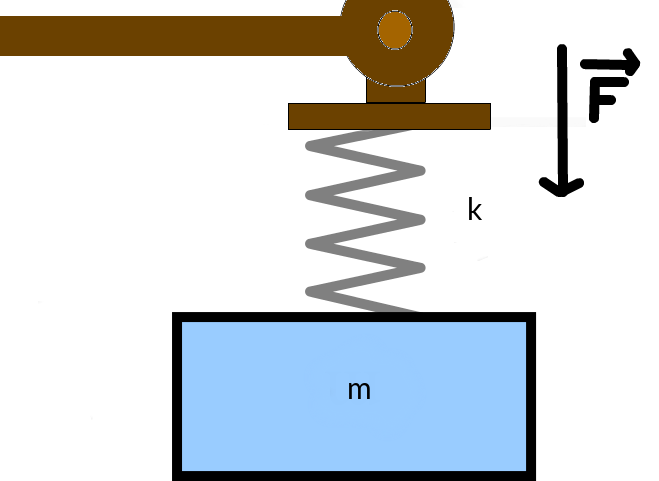
\includegraphics[scale=.3]{imagens/ForcedMass_spring.png}
                    \caption{Imagem meramente ilustrativa de um sistema massa-mola forçado}
                    \label{fig:forcedMMS}
                \end{figure}
                
                A solução analítica geral desse caso se dá por
                \begin{align}
                    u(t) &= c_1\cos{\omega_0t} + c_2\sin{\omega_0t} + u_p(t) \\\text{ com		}
                    \label{solPart}
                    u_p(t) &= t^s[A\cos{\omega t} + B\sin{\omega t}]
                \end{align}
                sendo $c_1$ e $c_2$ constantes da solução geral e $\omega_0$ a frequência natural do sistema. O termo $u_p(t)$ é a solução particular (também chamada solução transiente \cite{boyce9}) do problema na qual $s$ é ``o menor inteiro não negativo que garanta que nenhuma parcela de $u_p(t)$ seja solução da equação homogênea correspondente [...]'' \cite{regiIntro} e $A$ e $B$ são coeficientes da solução que podem ser determinados pelo método de coeficientes a determinar, como pode ser visto em \cite{regiIntro}.
                
                O código a seguir resolve, matematica e numericamente, o mesmo sistema massa-mola apresentado no exemplo anterior, porém agora com uma força externa agindo sobre o mesmo. A força externa $F_{ext}$ é descrita por
                \begin{equation*}
                    F_{ext} = \cos{\omega_0t}
                \end{equation*}
                \lstinputlisting[firstline=57,caption=Código da resolução numérica de um problema envolvendo um sistema massa-mola forçado]{Codigos/testeMassaMolaForcado.py}
                cujo resultado é exibido na Figura \ref{fig:MMforcado}
                \begin{figure}[H]
                    \centering 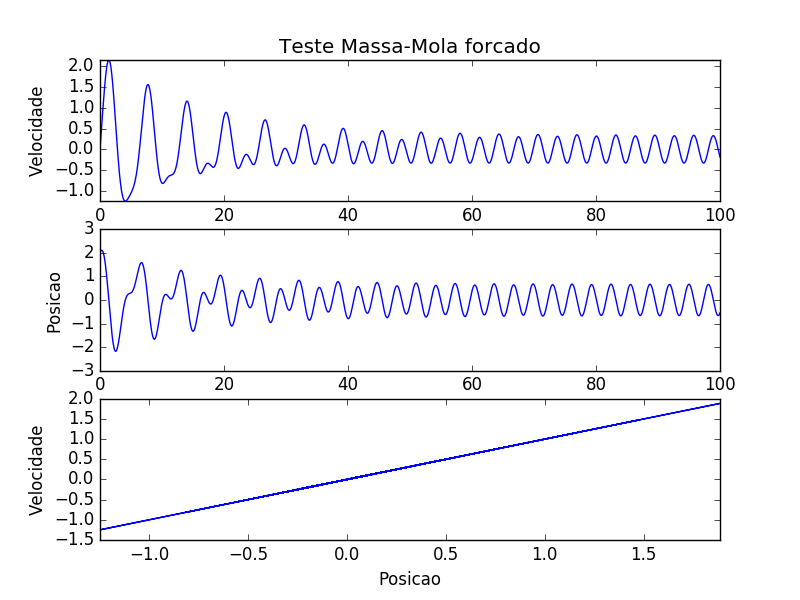
\includegraphics[scale=.54]{imagens/testeMassaMolaForcado.png}
                    \caption{Gráficos da posição e da velocidade da massa do sistema ao longo do tempo, seguido de um gráfico da velocidade pela posição}
                    \label{fig:MMforcado}
                \end{figure}
                
                O primeiro gráfico descreve a velocidade $v$ ao longo do tempo $t$ e o segundo descreve a posição $y$ da massa ao longo de $t$ também. Podemos perceber a ação da solução transiente até cerca de 50 unidades de tempo em ambos os gráficos, sendo que permanece depois apenas a solução geral (também chamada solução estado estacionário - \cite{boyce9}).
                
                O terceiro gráfico descreve a velocidade $v(t)$ em função da posição $y(t)$ da massa. O sinal da velocidade indica o sentido dela.